\documentclass{beamer}

\usepackage[utf8]{inputenc}
\usepackage{t1enc}
\usepackage[magyar]{babel}

\usepackage{lmodern}
\usepackage{amsmath}


\usetheme{default}



\setbeamertemplate{navigation symbols}{}

\usecolortheme{whale}

\definecolor{szechenyiblue}{RGB}{35, 76, 171} % define Széchenyi blue

\setbeamercolor*{title}{fg=white}
\setbeamercolor*{author}{fg=white}
\setbeamercolor*{date}{fg=white}
\setbeamercolor*{institute}{fg=white}
\setbeamercolor*{thanks}{fg=white}
\setbeamercolor*{frametitle}{bg=szechenyiblue, fg=white}


\makeatletter
\setbeamertemplate{title page}
{
	\vbox{}
	\begin{centering}
		
		\begin{beamercolorbox}[sep=8pt,center]{title}
			\usebeamerfont{title}\inserttitle    
		\end{beamercolorbox}%
		\begin{beamercolorbox}[sep=8pt,left]{author}
			\usebeamerfont{author}\insertauthor
		\end{beamercolorbox}
		\begin{beamercolorbox}[sep=8pt,left]{institute}
			\usebeamerfont{institute}\insertinstitute
		\end{beamercolorbox}
		\begin{beamercolorbox}[sep=8pt,left]{date}
			\usebeamerfont{date}\insertdate
		\end{beamercolorbox}
		\vspace{4em}
		\begin{beamercolorbox}[sep=2pt,left]{thanks}
			\usebeamerfont{date}\insertthanks
		\end{beamercolorbox}
		
	\end{centering}
}
\makeatother

\author{Kántor Attila, Grad-Gyenge László}
\title{\Huge{Szemantikus reprezent\'{a}ci\'{o} magyar nyelv eset\'{e}n}}
\institute[ELTE]

\date{\small{\today}}
\newcommand{\insertthanks}{\footnotesize{%
		A projekt az Európai Unió támogatásával,\\ az Európai Szociális Alap
		társfinanszírozásával\\ valósult meg\\ (\texttt{EFOP-3.6.3-VEKOP-16-2017-00002}).
}}




\begin{document}
	  

{
\usebackgroundtemplate{
\includegraphics[width=1.0\paperwidth]{szechenyi.jpg}}
	\begin{frame}[plain]
		\maketitle
	\end{frame}
}

\begin{frame}{Motiváció}

\begin{itemize}
	\item Természetesnyelv-feldolgozás részterülete
	\item Nyelvi elemek numerikus ábrázolása (szólista $\rightarrow$ vektortér)
	\item Modern módszerek meghatározó elemei:
	\begin{itemize}
		\item Alapjául szolgáló neurális háló (általában rekurrens vagy rekurzív)
		\item Tanítási feladatok és adathalmazok
	\end{itemize}
	\item Jó reprezentáció esetén közel kerülnek az azonos jelentésű vektorok egymáshoz
\end{itemize}

\end{frame}

\begin{frame}{Motiváció}
	
	\begin{itemize}
		\item Az így kapott vektorok számos módon felhasználhatók (osztályozás, keresőmotorok, chatbot)
		\item Léteznek többnyelvű megoldások, de a többség nyelvfüggő
		\item A modellek tanításához nagy mennyiségű adat szükséges
		\item Ember által címkézett adat $\rightarrow$ pontosabb eredmény
		\item Kis és közepes nyelvek (magyar) problémája: limitált eszköztár (csak felügyelet nélküli tanítás)
		\item Meglévő magyar nyelvű módszerek
		\begin{itemize}
			\item Csak szavak szintjén $\rightarrow$ kevésbé pontos
			\item Nincs lehetőség egyetlen modell segítségével nagyobb nyelvi elemek feldolgozására
		\end{itemize}
	\end{itemize}
	
\end{frame}

\begin{frame}{Előzmények}
	
\begin{itemize}
	\item Szóbeágyazási módszerek (szó $\rightarrow$ vektor)
	\begin{itemize}
		\item Word2Vec, GloVe
		\item Lokális és/vagy globális statisztikák
	\end{itemize}
	\item InferSent: Ember által annotált adat $\rightarrow$ jobb teljesítmény
	\item BERT: Autoannotált adattal is State-of-the-art eredmények
	\item USE: Kevés adat esetén jó megoldás lehet a transfer learning módszere
\end{itemize}
	
\end{frame}

\begin{frame}{Felhasznált adathalmazok}
	
\begin{itemize}
	\item A magyar nyelven elérhető tanítóhalmazok és források száma igen csekély (publikus korpuszok, web)
	\item OSCAR (40GB, csak a felét használtam) - publikus
	\begin{itemize}
		\item A Common Crawl tisztított és klasszifikált változata
		\item A mondatok nem sorrendtartóak
	\end{itemize}
	\item Hungarian Webcorpus (6,5 GB) - publikus
	\begin{itemize}
		\item Eredendően magyar nyelvű adathalmaz
		\item Kb. 1,2 millió magyar weboldal
	\end{itemize}
	\item Vásárlói vélemények (95 000 bejegyzés)
	\begin{itemize}
		\item Saját halmaz (Árukereső), vélemény - csillagok száma párosok
		\item 1-2 csillag $\rightarrow$ $-$, 4-5 csillag $\rightarrow$ $+$
		\item Tisztítva, egyensúlyozva
	\end{itemize}
\end{itemize}
	
\end{frame}

\begin{frame}{Az előtanítás - Architektúra}
	

\begin{columns}[t]
	\begin{column}{0.3\textwidth}
		\vspace{\topsep}
		
		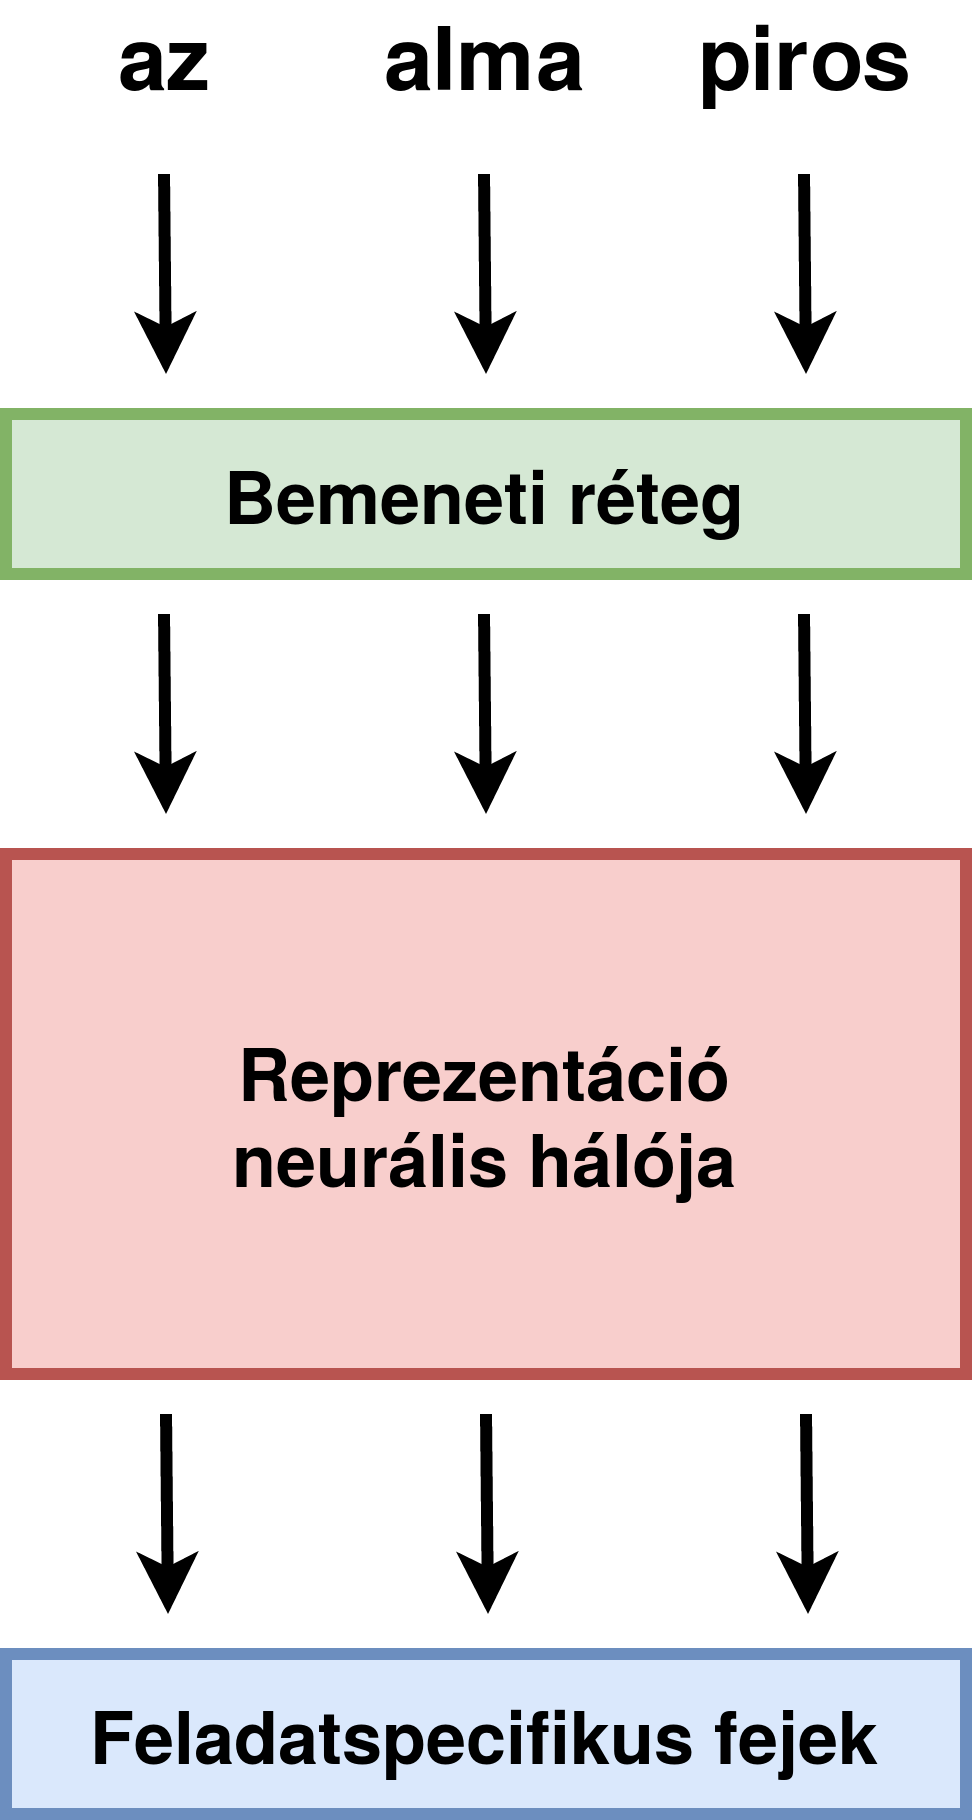
\includegraphics[width=\columnwidth]{architecture}%
	\end{column}
	
	\begin{column}{0.5\textwidth}
		\begin{itemize}
			\item Generált bemenet a Hungarian Webcorpus-ból
			\item Bemeneti tokenszekvencia Word2Vec vektorai (OSCAR - 645 000 méretű szótár)
		\end{itemize}
	\end{column}
\end{columns}
	
\end{frame}

\begin{frame}{Az előtanítás}
	
\begin{columns}[t]
	\begin{column}{0.4\textwidth}
		\vspace{\topsep}
		
		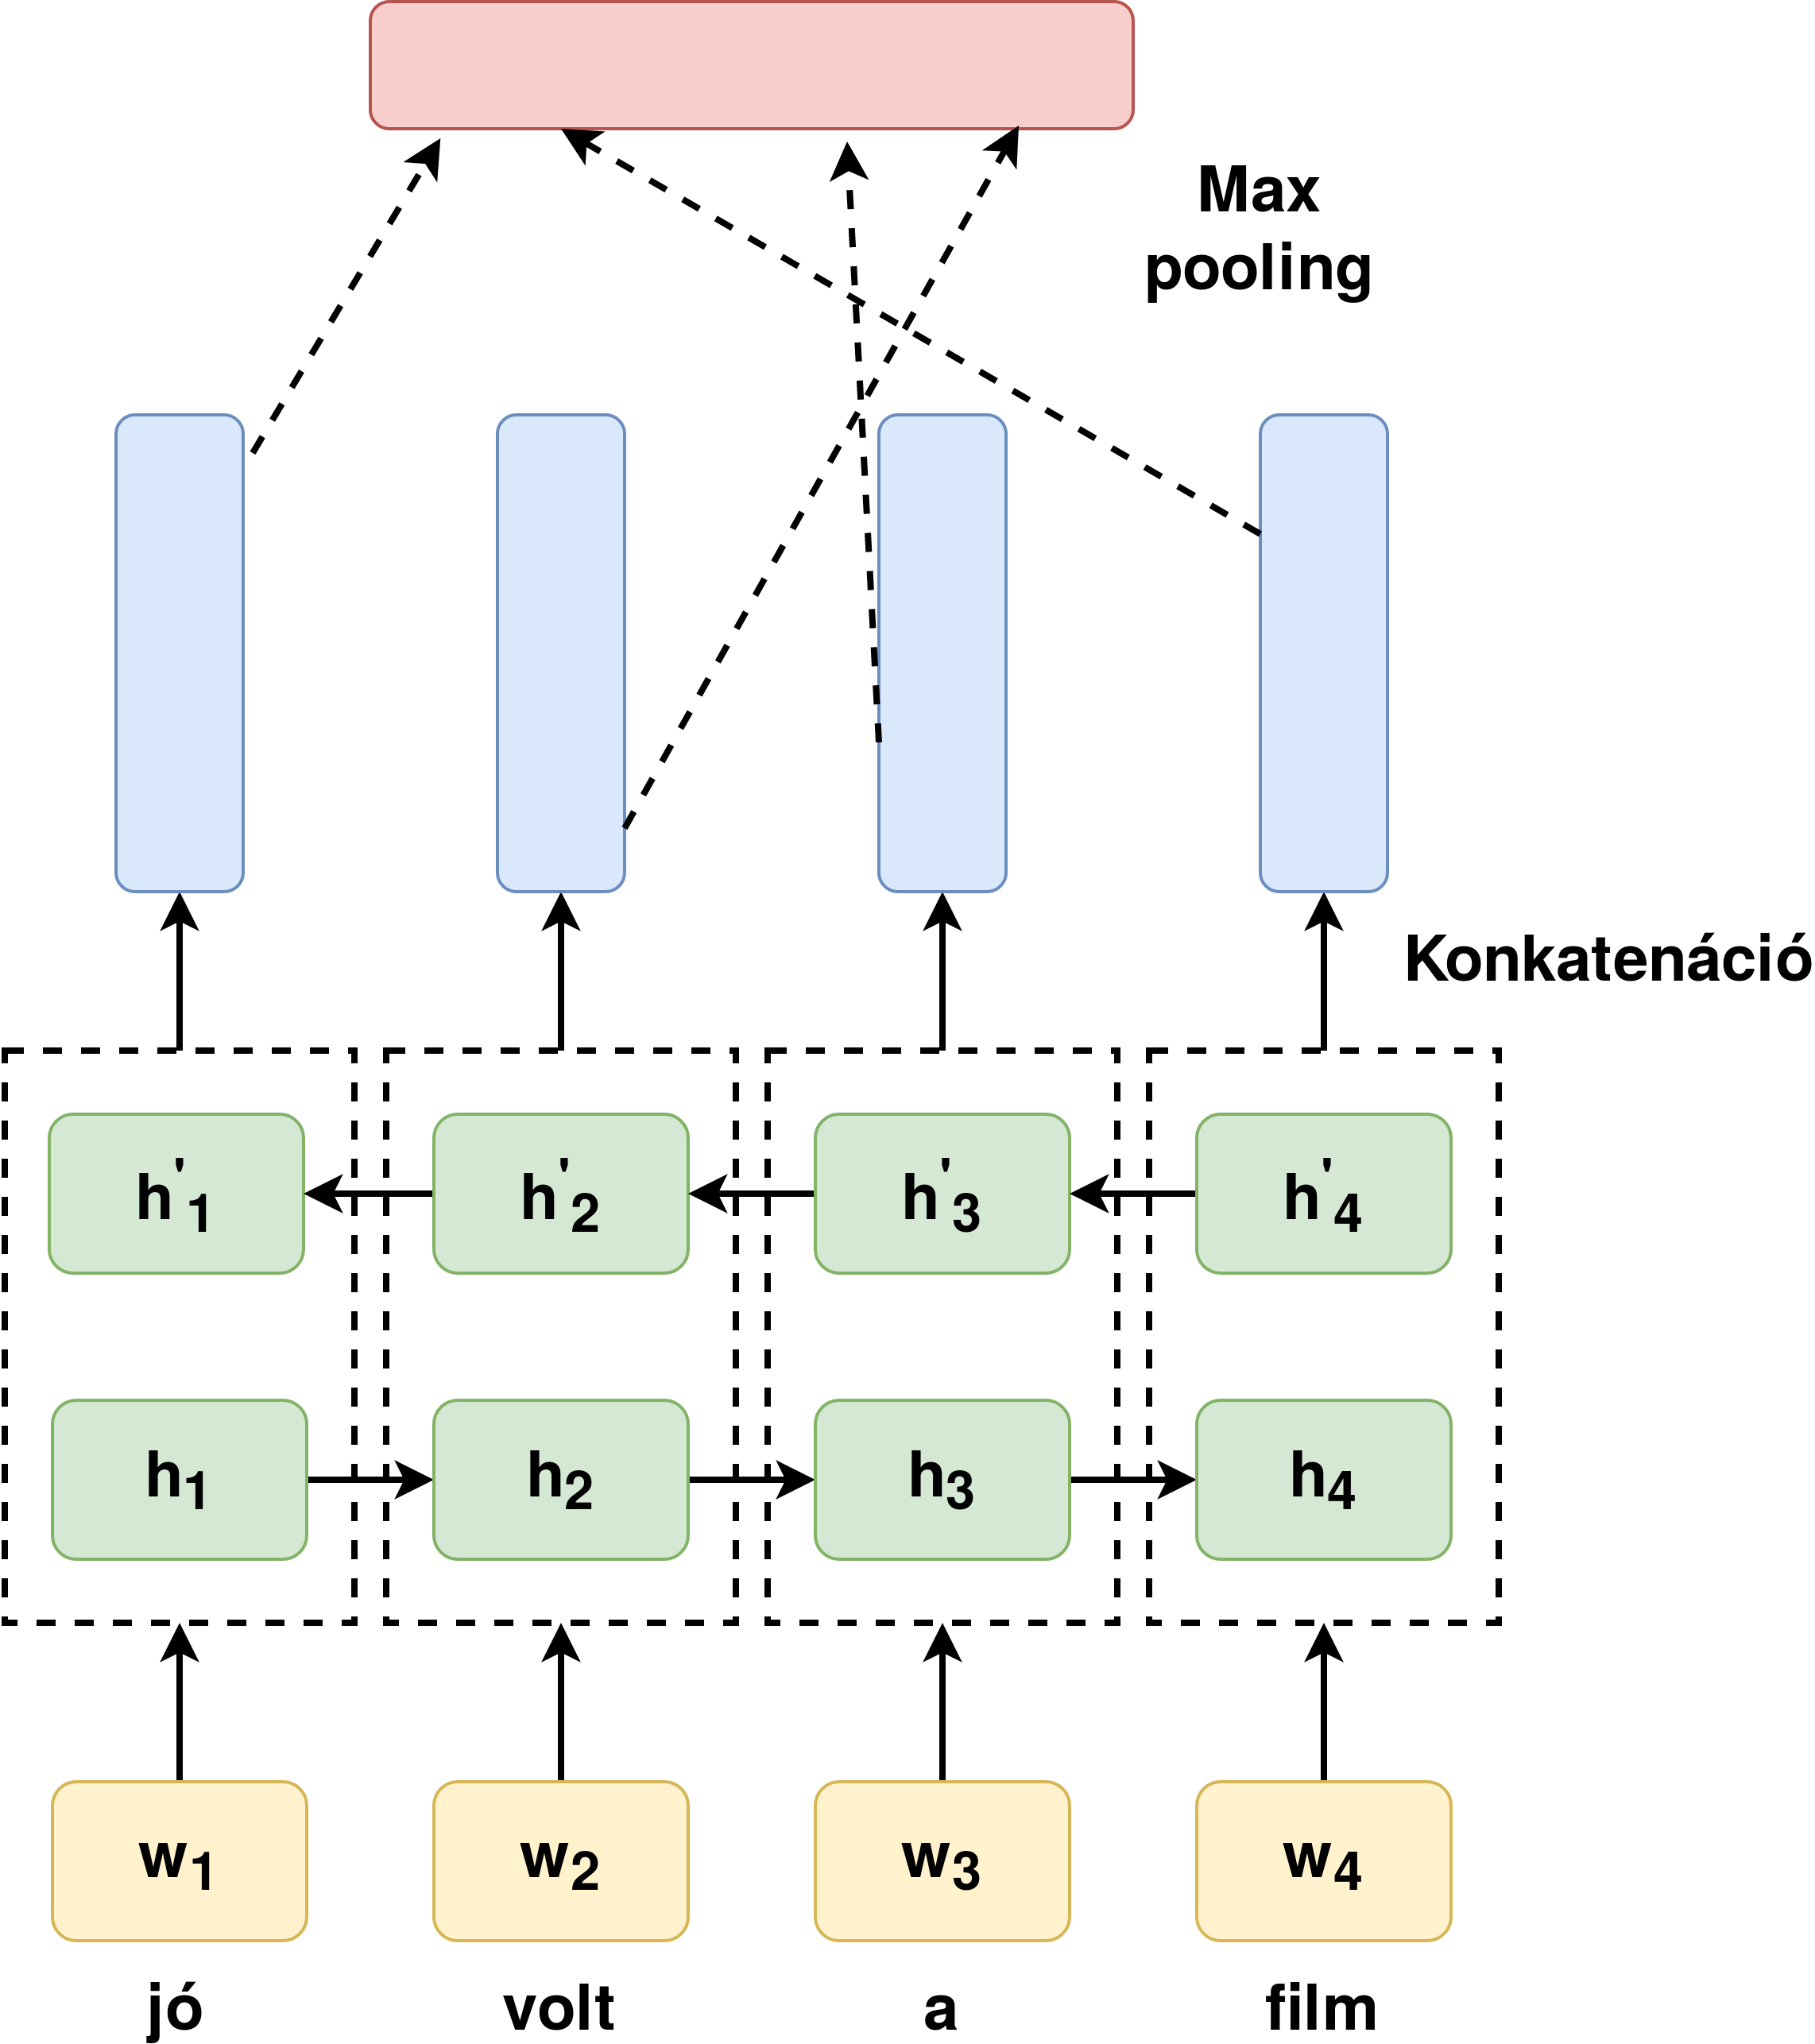
\includegraphics[width=\columnwidth]{biLSTM-max-pooling}%
	\end{column}
	
	\begin{column}{0.6\textwidth}
		\begin{itemize}
			\item BiLSTM max pooling (InferSent)
			\item Kétirányú olvasás
			\item Feladatok (BERT):
			\begin{itemize}
				\item \textbf{Maszkolás}: takarjuk le a szavak 15\%-át, a háló feladata kitalálni az eredeti tokeneket
				\item \textbf{Következő mondat}: A és B mondatok, vajon B szekvencia A után következik az eredeti dokumentumban?
			\end{itemize}
		\end{itemize}
	\end{column}
\end{columns}
	
\end{frame}

\begin{frame}{Az előtanítás}
	
\begin{itemize}
	\item Ismeretlen szavak problémája $\rightarrow$ saját dimenzió
	\item Normált bemenet $\rightarrow$ jobb teljesítmény
	\item LSTM rejtett méret növelése
\end{itemize}


	\begin{table}
		\centering
		\begin{tabular}{ | c | r | r | r |}
			\hline
			\textbf{Rejtett méret} & \textbf{Maszkolás} & \textbf{Következő mondat} \\
			\hline \hline		
			1024 & 16.61\% & 60.49\% \\
			\hline
			4096 & \textbf{17.82\%} & \textbf{94.15\%} \\
			\hline
		\end{tabular}
		\caption{Az előtanítás teszt pontossága}

	\end{table}
	
	
\end{frame}




\begin{frame}{A módszer kiértékelése}
	
\begin{itemize}
	\item A jó kiértékelési feladat jellemzői:
	\begin{itemize}
		\item Kellően nehéz, jól láthatóak a különbségek
		\item Jól interpretálható végeredmény
	\end{itemize}
	\item Vásárlói vélemények bináris klasszifikációja érzelmi tartalom alapján megfelelő
	\item Viszonyítási alap: Word2Vec vektorok átlaga
	\item Mérés menete: mondatvektorok generálása $\rightarrow$ osztályozó algoritmus $\rightarrow$ eredmény kimérése teszthalmazon
\end{itemize}	
	
\end{frame}


\begin{frame}{A módszer kiértékelése}
	
	\begin{table}
		\centering
		\begin{tabular}{ | c | r | r | r | r | r | r | r |}
			\hline
			\textbf{Modell / Osztályozó} & \textbf{Linear SVM} & \textbf{XGBoost} & \textbf{Random Forest} \\
			\hline \hline		
			\textbf{w2v\_sm} & 85,45\% & 82,18\% & 83,64\% \\
			\hline
			\textbf{w2v\_sm\_norm} & 85,57\% & 82,71\% & \textbf{84,18\%} \\
			\hline
			\textbf{w2v\_lg} & 85,28\% & 82,87\% & 83,77\% \\
			\hline
			\textbf{w2v\_lg\_norm} & 85,59\% & 83,15\% & 83,85\% \\
			\hline  
			\textbf{lstm\_1024} & 81,53\% & 80,82\% & 80,84\% \\
			\hline  
			\textbf{lstm\_1024\_norm} & 85,37\% & 83,48\% & 83,41\% \\
			\hline
			\textbf{lstm\_4096\_norm} & \textbf{87.16\%} & \textbf{83,71\%} & 83,90\% \\
			\hline
		\end{tabular}
		\caption{A modellek klasszifikációs pontossága a vélemények adathalmazon végzett bináris osztályozási feladat esetén. A w2v\_sm az oscar\_sm, a w2v\_lg az oscar halmazon tanított modelleket, a norm posztfix a normált bemenetet jelöli. A számok a modellek nevében a reprezentációs vektor méretére utalnak.}
	\end{table}
	
\end{frame}

\begin{frame}{További fejlesztések - a dolgozat nem tartalmazza}
	
\begin{itemize}
	\item Ismeretlen tokenek 0 súlyozása a maszkolási feladat esetén $\rightarrow$ teljesítmény romlott
	\item lstm\_4096\_norm modell finomhangolása a vélemények adathalmazon $\rightarrow$ jelentős javulás (89,67 \% teszt pontosság)
\end{itemize}
	
\end{frame}

\begin{frame}{Összefoglaló}
	
A dolgozat tartalma:
	
\begin{itemize}
	\item Angol nyelvű módszerek és magyar nyelvű korpuszok vizsgálata
	\item Egy előre tanított magyar nyelvű kétirányú reprezentációs modell létrehozása mondatokra és paragrafusokra
	\item Mérési adathalmaz magyar nyelvű reprezentációs módszerekhez
	\item A bemutatott algoritmus az adott feladat esetén túlteljesítette a Word2Vec-et
\end{itemize}
	
\end{frame}



%\begin{frame}{Motiváció}
	%Törzsszöveg kinézete
	
	%\begin{block}{Definiált kifejezés}
	%	Definíció szövege
%	\end{block}

%	\begin{exampleblock}{Megjegyzés fejléce}
	%	Megjegyzés szövege
%	\end{exampleblock}

%	\begin{alertblock}{Figyelmeztetés!}
%		Erre nagyon figyelj oda!
%	\end{alertblock}
%\end{frame}



{
	\usebackgroundtemplate{
\includegraphics[width=1.0\paperwidth]{szechenyi.jpg}}
	\begin{frame}[plain]
		\begin{center}
			\textcolor{white}{\Huge{Köszönöm a figyelmet!}}
		\end{center}
	\end{frame}
}



	
\end{document}
